\documentclass[10pt,conference,a4paper]{IEEEtran}
\usepackage[utf8]{inputenc}
\usepackage{graphicx}
\usepackage{float}
\usepackage{enumerate}
\usepackage[spanish]{babel}
\usepackage[hidelinks]{hyperref}

%opening
\title{[ELO313] Procesamiento Digital de Se\~nales\\ 
Tarea I}
\author{Cristian Acuña S.{\small $~^1$}
\vspace{1.6mm}\\
Departamento de Electrónica, Universidad Técnica Federico Santa María.\\
	Avenida España 1680, Valparaíso, Chile.\\
	\fontsize{9}{9}\selectfont\ttfamily\upshape

	$~^{1}$\,cristian.acuna@alumnos.usm.cl (2921006-3)
}
\date{6 de Mayo de 2014}

\begin{document}

\maketitle

\section{Evaluaci\'on de Propiedades de Sistemas}

Se pide verificar las propiedades de invariancia en el tiempo, linealidad y 
causalidad para ciertos sistemas desconocidos \verb|bbox1|, \verb|bbox2| y 
\verb|bbox3|.

\subsection{Invariancia en el tiempo}

Para probar esta propiedad, los sistemas son estimulados con pulso cuadrado de 
largo total 30 ($\mu[n-10]-\mu[n-20]$), y luego estimulados con la misma 
se\~nal con un retraso temporal ($\mu[n-15]-\mu[n-25]$). Para dichos sistemas, 
se presentan los resultados de estos est\'imulos en las figuras 
(\ref{fig:img1}), (\ref{fig:img2}) y (\ref{fig:img3}) respectivamente.

\begin{figure}[H]
  \centering
  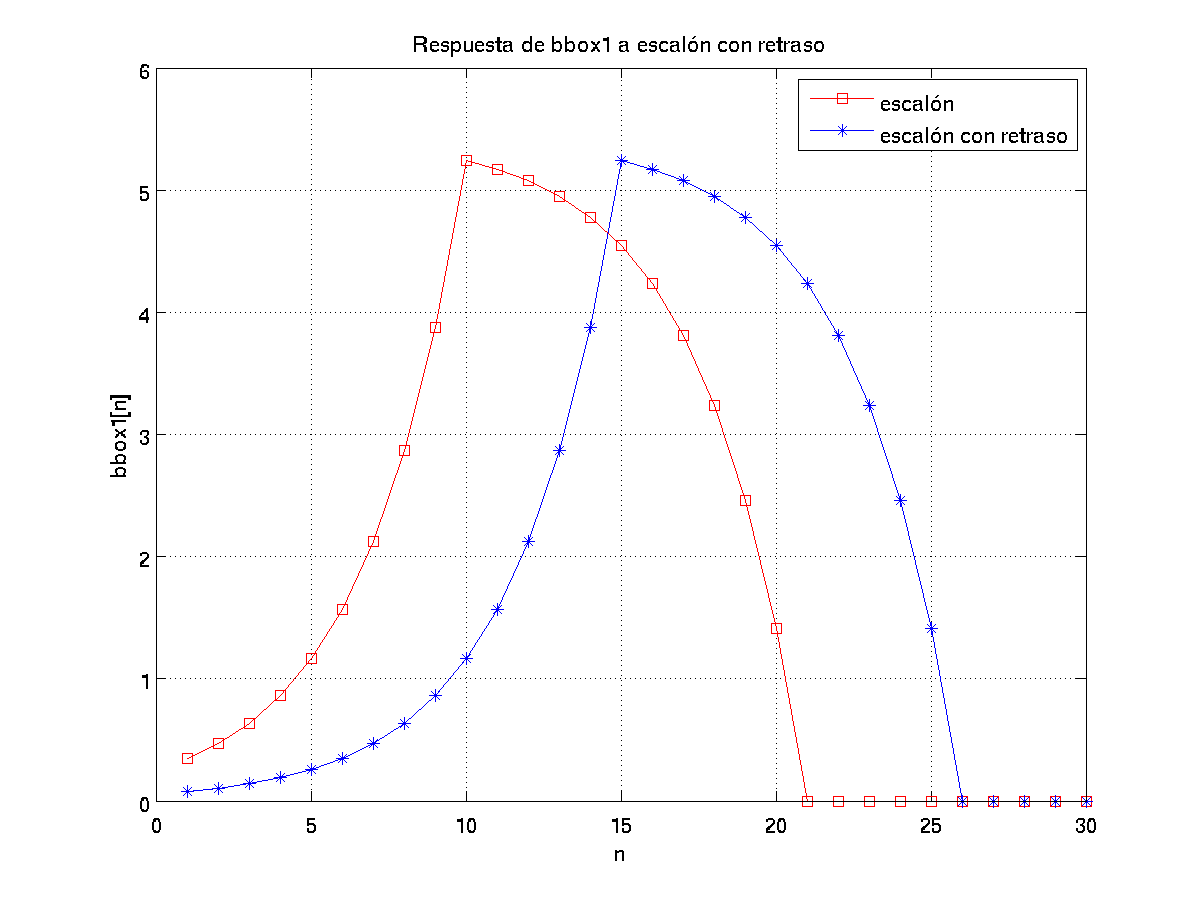
\includegraphics[width=0.45\textwidth]{../img/img1.png}
  \caption{Respuesta de bbox1.}
  \label{fig:img1}
\end{figure}

\begin{figure}[H]
  \centering
  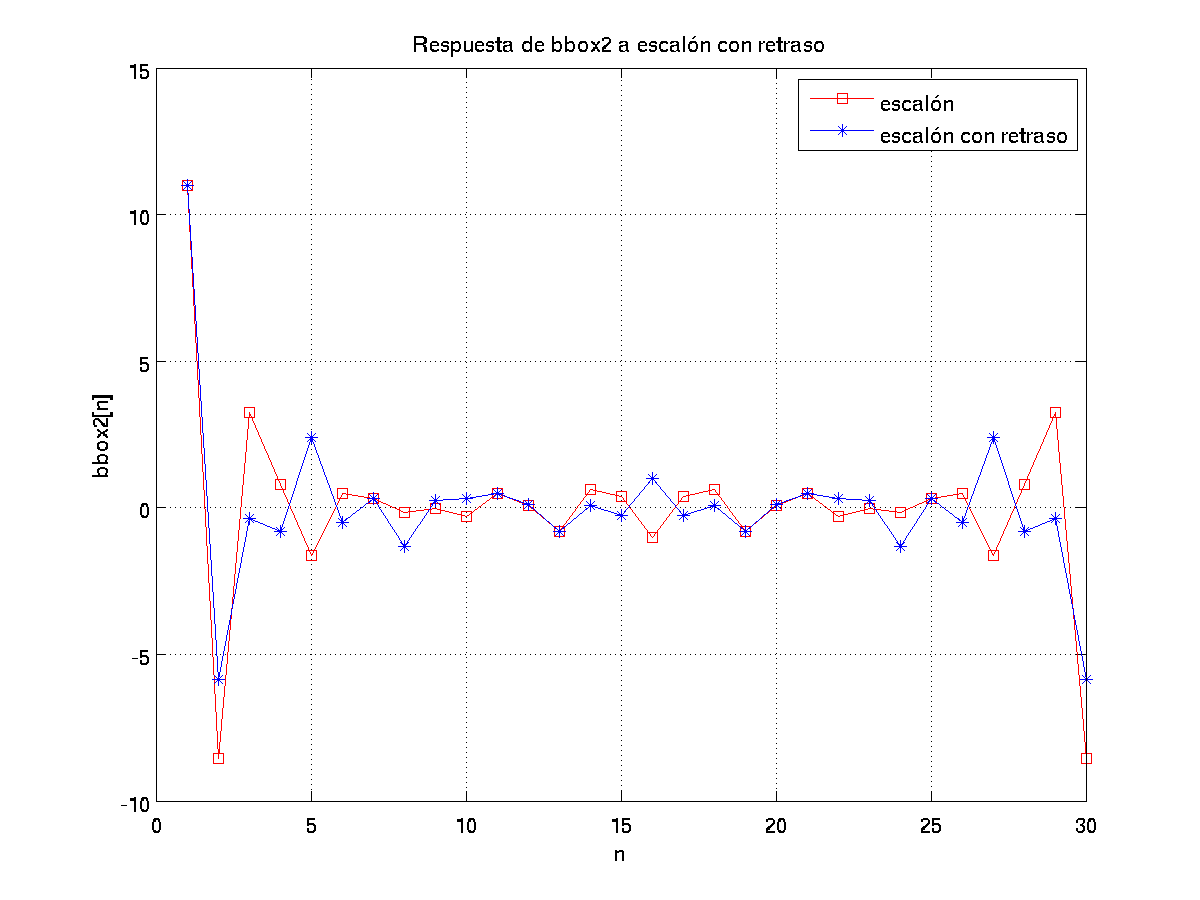
\includegraphics[width=0.45\textwidth]{../img/img2.png}
  \caption{Respuesta de bbox2.}
  \label{fig:img2}
\end{figure}

\begin{figure}[H]
  \centering
  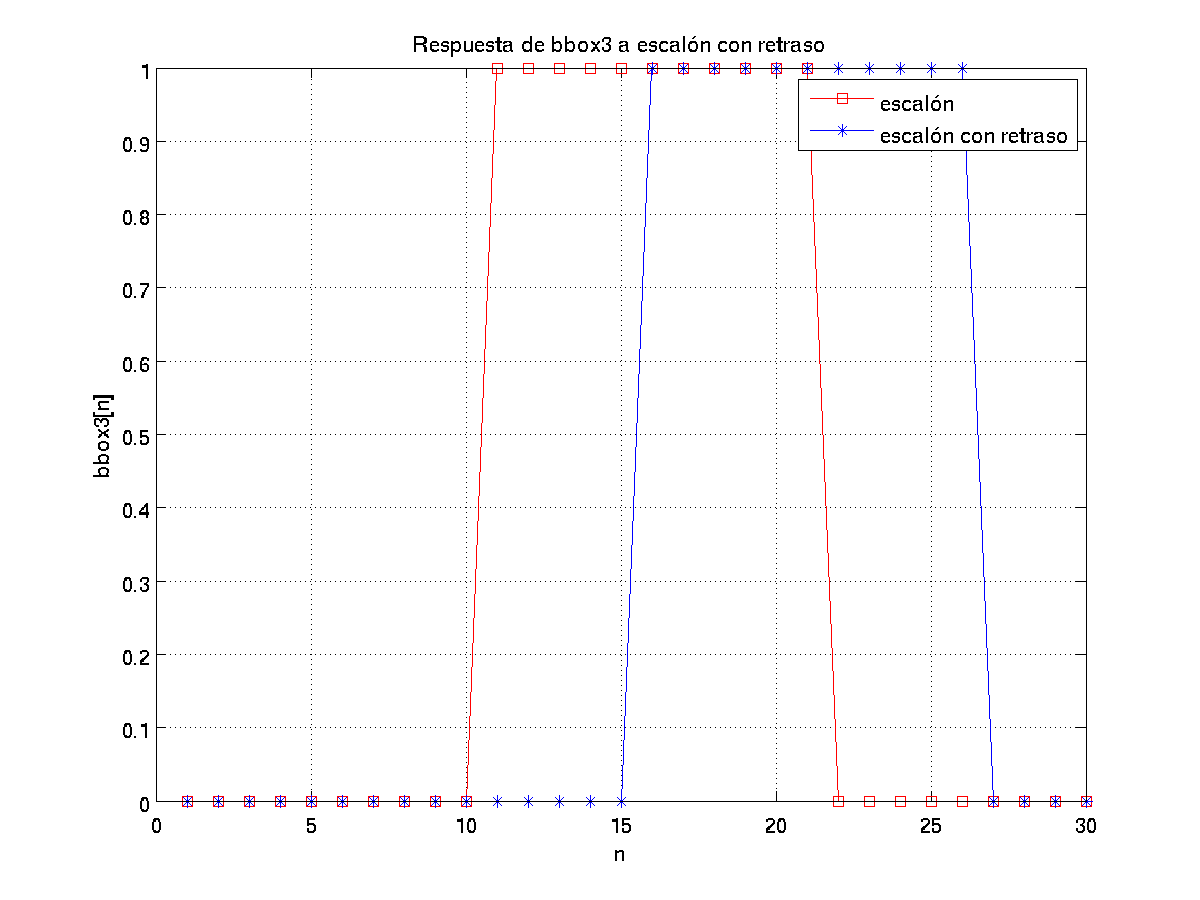
\includegraphics[width=0.45\textwidth]{../img/img3.png}
  \caption{Respuesta de bbox3.}
  \label{fig:img3}
\end{figure}

Se puede apreciar en la figura (\ref{fig:img2}) que la respuesta de \verb|bbox2|
ante una se\~nal no es la misma se\~nal retrasada. En este caso corresponde a 
una se\~nal diferente. Por lo tanto, se puede concluir que \verb|bbox2| es un 
sistema que var\'ia con el tiempo.

\subsection{Linealidad}



\end{document}
